\documentclass[11pt]{article}

\usepackage{amsmath}
\usepackage{amsfonts}
\usepackage[margin=1in]{geometry}
\usepackage{enumitem}
\usepackage{graphicx}
\usepackage[colorlinks]{hyperref}
\usepackage{longtable}

\usepackage{helvet}
\renewcommand{\familydefault}{\sfdefault}

\setlength{\parindent}{0in}

\def\tightlist{}
\def\toprule{}
\def\bottomrule{}

\begin{document}
{\LARGE Homework 3 (Due September
23rd)}\label{homework-3-due-september-23rd}

Homework 3 emphasizes alternative methods to direct integration
(Coulomb's Law) for solving the electric field problem including the use
of Gauss' Law and reducing the vector problem to a scalar one by using
electric potential. In addition, it introduces the concept of the Dirac
delta function as a tool for describing distributions of charge. This
homework makes use of what you learned in Secs. 1.5, 2.2, and 2.3 (up to
about 2.3.2), but what you know from 2.1 (i.e., superposition of
(\(\mathbf{E}\)) will also be important.

\paragraph{1. Comparing Coulomb's Law to Gauss'
Law}\label{comparing-coulombs-law-to-gauss-law}

Now that we have, in principle, fully described how to solve any
electrostatics problem (i.e., by adding up the contribution of each
chunk of charge), we turn to building our theoretical toolbox by
learning alternative methods that make the solving of certain kinds of
problems more tractable. The first of these alternatives is Gauss' Law.
It is important to know when and how to apply Gauss' Law - in the
problem below, you are asked to compare Gauss' Law with Coulomb's Law.

Consider the following questions in finding the electric field
everywhere for a conducting sphere, a uniformly charged sphere, and a
sphere with charge distribution varying as \(r^n\), all with radius
\(r_0\) and total charge \(Q\):

\begin{enumerate}
\def\labelenumi{\arabic{enumi}.}
\tightlist
\item
  What are the advantages and disadvantages of using Gauss' Law to find
  the electric field instead of using Coulomb's Law (Griffiths Eq 2.8)?
  What role does symmetry play?
\item
  Answer the same questions for three cubes with the same properties
  (i.e., charge distributions that vary radially as \(r^n\)).
\item
  What do your answers to parts 1 and 2 tell you about using Gauss' Law
  versus using Coulomb's Law (direct integration) to solve for the
  electric field?
\end{enumerate}

\paragraph{2. Spherical charge distributions are
special}\label{spherical-charge-distributions-are-special}

As you might have picked up by now, spherically symmetric charge
distributions are very special. We have a number of theoretical tools we
can bring to bear on them and the results we produce are often quite
simple in a mathematical sense. In this problem, you will explore these
distributions a bit more and connect the mathematics (i.e., the
integrals you must do) to the geometry of the problem (i.e., where the
charge lives) to gain intuition about these spherically symmetric
distributions of charge.

For parts 1 and 2, consider a sphere of radius \(R\), centered one the
origin, with a radially symmetric charge distribution \(\rho(r)\).

\begin{enumerate}
\def\labelenumi{\arabic{enumi}.}
\tightlist
\item
  What \(\rho(r)\) is required for the electric field \textbf{in the
  sphere} to have the power law form \(E(r) = cr^n\), where \(c\) and
  \(n\) are constants? The case of n=-2 is special. How so? Some values
  of \(n\) are unphysical because these would lead to an infinite amount
  of charge in the sphere.. Which values of \(n\) are allowed?
\item
  What kind of charge distribution is required for the radial E-field
  inside the sphere to be of constant magnitude; that is, what
  \(\rho(r)\) produces \$E(r) = \$ constant (inside only)? Is this
  distribution physical realizable? Why or why not?
\item
  For each of these allowable charge distributions, what does the
  electric field look like outside the sphere (\(r>R\))?
\item
  \emph{The following problem is from the 2001 Physics GRE Exam.
  Students were expected to solve the problem in just a few minutes!}
  Two spherical, nonconducting, and very thin shells of uniformly
  distributed positive charge \(Q\) and radius \(d\) are located a
  distance 10\(d\) apart. A positive point charge \(q\) is placed inside
  on of the shells at a distance \(d/2\) from the center, on the line
  connecting the centers of the two shells, as shown in the figure. What
  is the net force on the charge \(q\)?
\end{enumerate}

\begin{figure}[htbp]
\centering
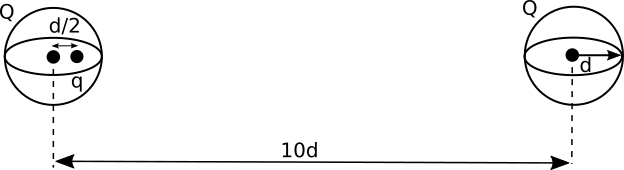
\includegraphics{./images/hw3/gre_problem.png}
\caption{GRE Problem}
\end{figure}

\paragraph{3. Overlapping clouds of
charge}\label{overlapping-clouds-of-charge}

When solving some E\&M problems, you will need to develop your argument
(i.e., you solution) using an arbitrary location. In this problem,
consider how choosing an arbitrary point in the overlapping region of
the charge clouds will help you derive the result.

\begin{figure}[htbp]
\centering
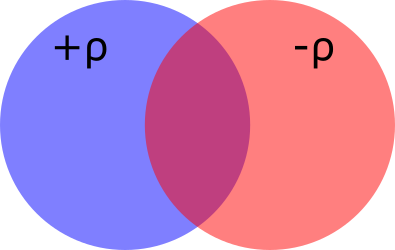
\includegraphics{./images/hw3/overlapping_clouds.png}
\caption{Overlapping Clouds}
\end{figure}

\begin{enumerate}
\def\labelenumi{\arabic{enumi}.}
\tightlist
\item
  For a cloud of charge (radius, \(R\)) with uniform charge density
  (\(\rho_0\)), determine the electric field inside and outside the
  cloud.
\item
  Graph the electric field as a function of distance from the center of
  the cloud. \href{../jupyter/HW3-LinePlotting.ipynb}{Download this
  Jupyter notebook} to create this plot (you can
  \href{https://github.com/dannycab/phy481msu/blob/gh-pages/jupyter/HW3-LinePlotting.ipynb}{view
  it here}). \emph{You will have to choose values for \(\rho_0\) and
  \(R\) to make your graph.}
\item
  Consider two oppositely charged clouds (radii, \(R\)), both with
  uniform charge densities. They overlap like shown in the figure with
  their centers separated by \(d\). Find the electric field in the
  overlapping region. (\emph{Hint: consider how Gauss' Law and
  superposition can help here.})
\item
  In this overlapping region, sketch the electric field lines.
\item
  In the limit that \(d\) becomes very small compared to \(R\), discuss
  in words and make a sketch of what the resulting (total, physical)
  charge distribution in space really looks like (so that later in the
  course when we encounter such a charge distribution, we will know
  where it came from and what the electric field looks like inside!)
\end{enumerate}

\paragraph{4. Cube with a hole}\label{cube-with-a-hole}

What happens when you have problems were the symmetries are mixed? How
do you tackle a problem with two different geometries? In this problem,
you will explore how to deal with situations where they are two
``competing'' geometries for the problem. Sometimes you will need to
bring two (or more!) aspects of your theoretical toolbox to bear on a
problem.

Consider a cube (edge length \(a\)) with a uniform charge distributed
throughout its volume (\(\rho\)). We carve a spherical cavity out of it
of radius \(d\), such that the cavity is centered at the center of the
cube.

\begin{figure}[htbp]
\centering
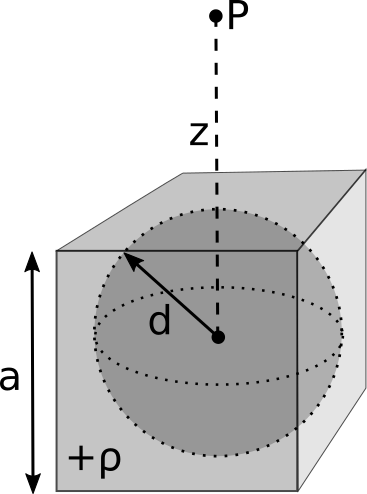
\includegraphics{./images/hw3/cube_w_hole.png}
\caption{Cube with Hole}
\end{figure}

\begin{enumerate}
\def\labelenumi{\arabic{enumi}.}
\tightlist
\item
  Does Gauss' Law hold for this problem? Can Gauss' Law be used on this
  problem? If so, what surface do you use? If not, why?
\item
  Let the center of the cube (and thus the center of the cavity) be
  located at the origin \(\langle 0,0,0 \rangle\). \textbf{Explain} how
  you would determine the electric field at point \(P\) a distance \(z\)
  from the center of the cube.
\item
  What should your expression for the electric field be as \(d\) goes to
  zero. What does this correspond to physically?
\end{enumerate}

\paragraph{5. Describing charge distributions with delta
functions}\label{describing-charge-distributions-with-delta-functions}

The \href{https://en.wikipedia.org/wiki/Dirac_delta_function}{Dirac
delta function} is an important theoretical tool for describing
distributions of a variety of physical quantities (e.g., mass, charge)
where a point object (or system of point objects) is the model we intend
to use. In addition, it can be used to describe distributions where
these quantities exist in highly constrained spaces (e.g., on a plane or
spherical shell). In this class, we will use the Dirac delta function to
describe how a charges are distributed. In this problem, you will get
familiar with the Dirac delta function for a set point charges on a
line.

The linear charge density for a series of charges on the \(x\)-axis is
given by:

\[\lambda(x) = \sum_{n=0}^{10} q_0 n^2\delta\left(x-\dfrac{n}{10}\right)\]

\begin{enumerate}
\def\labelenumi{\arabic{enumi}.}
\tightlist
\item
  Write a sentence or two describing the units of each term in the
  equation. (Don't forget the delta function!)
\item
  What is the total charge on \(x\)-axis?
\end{enumerate}

\paragraph{6. Using Dirac delta functions in
electrostatics}\label{using-dirac-delta-functions-in-electrostatics}

Sometimes, we will describe the distribution of charge (\(\rho\)) using
the Dirac delta function. We will need to be able to use that
description to find the electric field (e.g., by using Coulomb's Law).
in this problem, you will work with the Dirac delta function to describe
point charge distributions with which you are familiar. You will also
find the electric field due to those charge distributions. We aim for
you to gain confidence in using Dirac delta functions by checking you
can find the field that you determine through other means.

\begin{enumerate}
\def\labelenumi{\arabic{enumi}.}
\tightlist
\item
  Write down the appropriate expression for the volume charge density,
  \(\rho(\mathbf{r})\), for a point charge, \(q\), located at
  \(\mathbf{r}'\). Interpret the units of each term in the expression.
\item
  Consider an electric dipole with a \(+q\) charge at a location \(+d\)
  on the \(y\)-axis and a \(-q\) charge located at \(-d\) on the
  \(y\)-axis. Write down the volume charge density, \(\rho(\mathbf{r})\)
  for this distribution.
\item
  Using Coulomb's law (direct integration), show that you can obtain the
  electric field of this dipole at any location \(x\) on the \(x\)-axis.
\item
  Write down the appropriate expression for the \emph{volume} charge
  distribution (\(\rho\)) for an infinite plane of charge at \(z = a\)
  with surface charge density \(\sigma_0\). Comment on the units of each
  term in your distribution.
\end{enumerate}

\paragraph{7. Connecting potential, electric field, and
charge}\label{connecting-potential-electric-field-and-charge}

It is common in theoretical physics to describe the interactions of a
system in terms of a scalar field (i.e., its potential). It is a compact
description and you can (if you are careful) derive other important
aspects of the system (e.g., how its sources are configured) from that
scalar field if there is a rule for doing so. In this problem, you will
do this work for a negative point charge. The understanding you draw
from this problem will be used in future problems where the electric
field and charge density might not be obvious.

Consider the potential of a point charge at the origin:

\[V(r) = -\dfrac{1}{4\pi\varepsilon_0}\dfrac{q}{r}\]

\begin{enumerate}
\def\labelenumi{\arabic{enumi}.}
\tightlist
\item
  Determine the electric field of this charge by calculating the
  gradient (\(\mathbf{E} = -\nabla V\)). Show your work.
\item
  Calculate the charge density from the electric field by using Gauss'
  Law directly
  (\(\nabla \cdot \mathbf{E} = \frac{\rho}{\varepsilon_0}\)). Do this 2
  ways: (1) Use the definition of the divergence from the front fly leaf
  of Griffiths in spherical coordinates (what do you get?) and (2) by
  performing a coordinate-free calculation (is your answer the same?).
\item
  How do your two answers from part 2 compare? Which one is correct? How
  do you know? What does this tell you about computing charge densities
  from electric potentials?
\end{enumerate}

For part 2, the following vector identities might be helpful:

\[\nabla \left(f(\mathbf{r}) \mathbf{A}\right) = \nabla f(\mathbf{r}) \cdot \mathbf{A} + f(\mathbf{r}) \nabla \cdot \mathbf{A}\]

\[\nabla \cdot \dfrac{\hat{r}}{r^2} = 4\pi\delta^3(\mathbf{r})\]

\[\nabla \cdot \dfrac{\hat{r}}{r} = \dfrac{1}{r^2}\]

\paragraph{8. Estimating the amount of excess charge on a
balloon}\label{estimating-the-amount-of-excess-charge-on-a-balloon}

Developing real world estimates of certain E\&M phenomenon is an
important skill to develop from this course. If what we do doesn't
describe reality, what's the point?! In this problem, you will develop
an estimate for that amount of electrons transferred to a balloon
through ``static electricity.''

An electric field strength of 300 kV/m can cause the molecules in the
air to breakdown allowing a spark to travel through the air. You have
probably rubbed a ballon through your hair and heard some crackling -
that is one effect of the breakdown of the molecules in the air as a
result of this high field strength due to transferred electrons.

\begin{enumerate}
\def\labelenumi{\arabic{enumi}.}
\tightlist
\item
  Estimate the minimum amount of static charge on a balloon that could
  cause this sparking. In your estimation, make clear any assumptions
  you are making and/or quantities that you are estimating or looking
  up. Explain how you are making this estimate in words.
\item
  Using your estimate in part 1, further estimate the fraction of excess
  electrons on the surface of the balloon compared to the number
  electrons that make up the balloon. Does this estimate seem reasonable
  to you? Why or why not?
\end{enumerate}
\end{document}
